\documentclass[tikz,border=8pt]{standalone}
\usepackage[utf8]{inputenc}
\usepackage[T1]{fontenc}
\usepackage{tikz}
\usetikzlibrary{arrows.meta,positioning,calc,decorations.pathreplacing}

\begin{document}
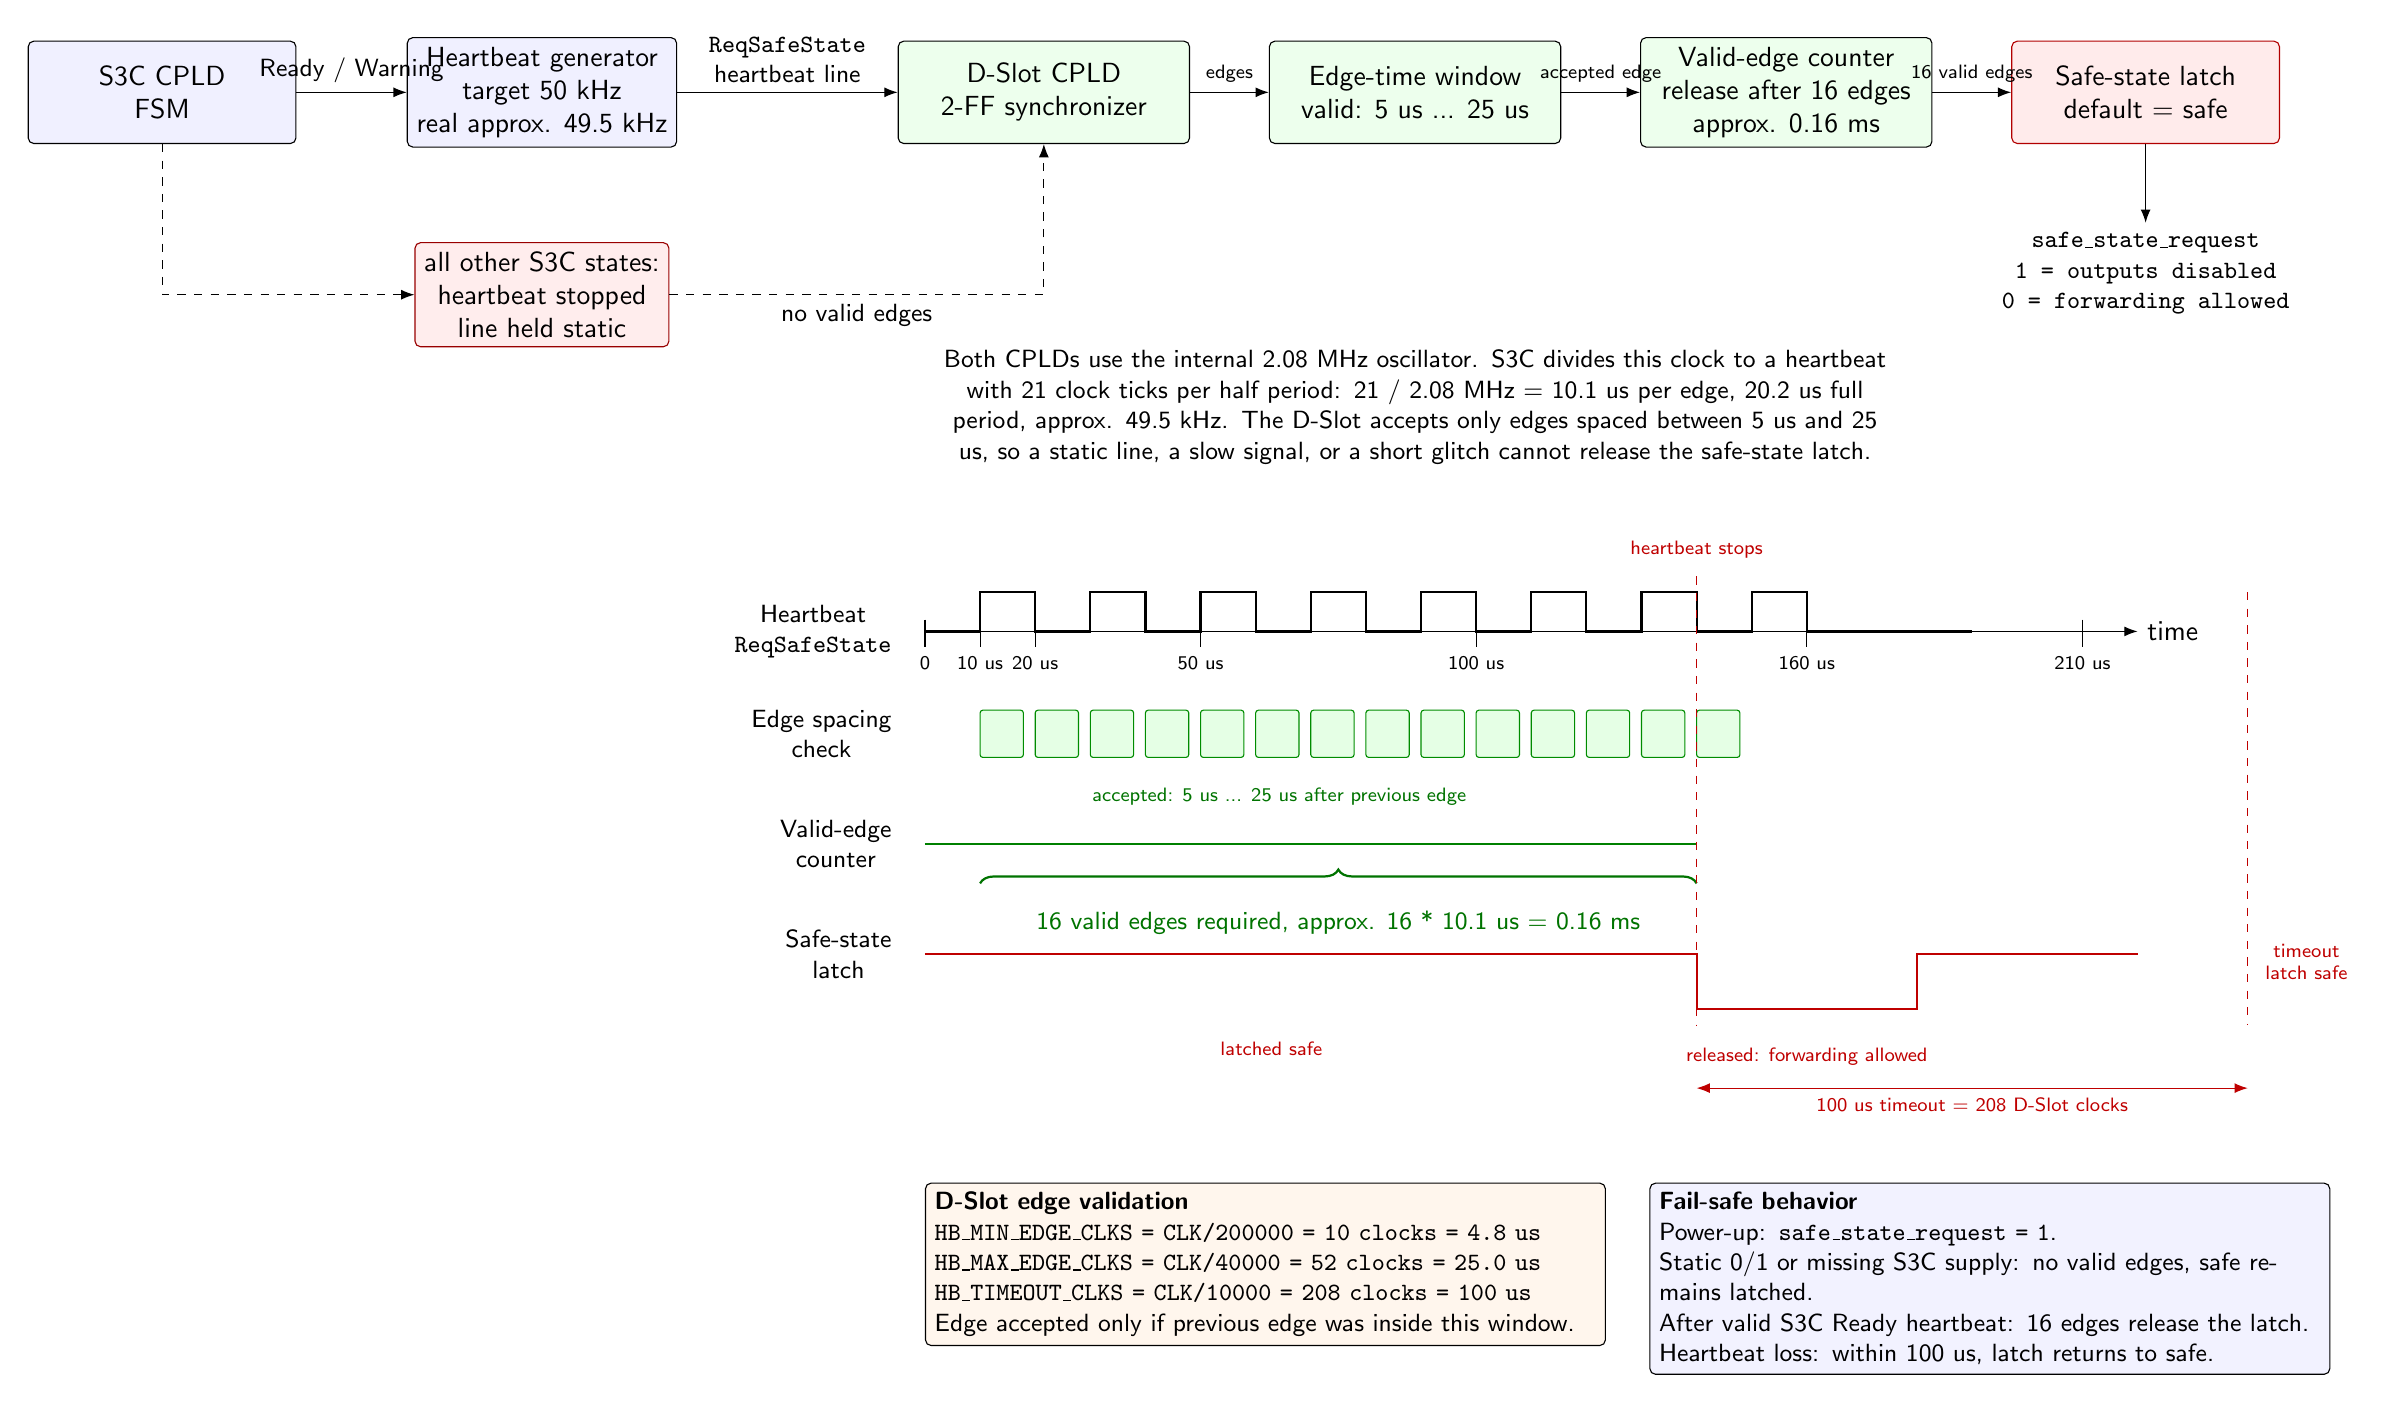
\begin{tikzpicture}[
  font=\sffamily,
  >=Latex,
  block/.style={draw, rounded corners=2pt, align=center, minimum height=13mm, minimum width=34mm, fill=blue!6},
  dblock/.style={draw, rounded corners=2pt, align=center, minimum height=13mm, minimum width=37mm, fill=green!7},
  latch/.style={draw=red!70!black, fill=red!8, rounded corners=2pt, align=center, minimum height=13mm, minimum width=34mm},
  warn/.style={draw=red!60!black, rounded corners=2pt, align=center, minimum height=11mm, fill=red!7},
  note/.style={align=center, font=\sffamily\small},
  tinytext/.style={align=center, font=\sffamily\scriptsize},
  sig/.style={thick},
  edgewin/.style={draw=orange!80!black, fill=orange!13, rounded corners=1pt},
  good/.style={draw=green!55!black, fill=green!10, rounded corners=1pt},
  bad/.style={draw=red!70!black, fill=red!9, rounded corners=1pt}
]

% ---------------------------------------------------------------------------
% Handshake block diagram
% ---------------------------------------------------------------------------
\node[block] (s3cfsm) {S3C CPLD\\FSM};
\node[block, right=14mm of s3cfsm] (hbgen) {Heartbeat generator\\target 50 kHz\\real approx. 49.5 kHz};
\node[dblock, right=28mm of hbgen] (sync) {D-Slot CPLD\\2-FF synchronizer};
\node[dblock, right=10mm of sync] (window) {Edge-time window\\valid: 5 us ... 25 us};
\node[dblock, right=10mm of window] (counter) {Valid-edge counter\\release after 16 edges\\approx. 0.16 ms};
\node[latch, right=10mm of counter] (latch) {Safe-state latch\\default = safe};

\draw[->] (s3cfsm) -- node[above,note] {Ready / Warning} (hbgen);
\draw[->] (hbgen) -- node[above,note] {\texttt{ReqSafeState}\\heartbeat line} (sync);
\draw[->] (sync) -- node[above,tinytext] {edges} (window);
\draw[->] (window) -- node[above,tinytext] {accepted edge} (counter);
\draw[->] (counter) -- node[above,tinytext] {16 valid edges} (latch);

\node[warn, below=12mm of hbgen] (stop) {all other S3C states:\\heartbeat stopped\\line held static};
\draw[->, dashed] (s3cfsm.south) |- (stop.west);
\draw[->, dashed] (stop.east) -| node[pos=.25,below,note] {no valid edges} (sync.south);

\node[note, below=10mm of latch] (out) {\texttt{safe\_state\_request}\\
\texttt{1 = outputs disabled}\\
\texttt{0 = forwarding allowed}};
\draw[->] (latch) -- (out);

\node[note, below=25mm of window, text width=122mm] (params) {
Both CPLDs use the internal 2.08 MHz oscillator. S3C divides this clock to a heartbeat with
21 clock ticks per half period: 21 / 2.08 MHz = 10.1 us per edge, 20.2 us full period,
approx. 49.5 kHz. The D-Slot accepts only edges spaced between 5 us and 25 us, so a
static line, a slow signal, or a short glitch cannot release the safe-state latch.
};

% ---------------------------------------------------------------------------
% Timing diagram, scaled in us
% scale: 1 us = 0.7 mm
% ---------------------------------------------------------------------------
\coordinate (t0) at ($(params.south west)+(0,-20mm)$);
\coordinate (tend) at ($(t0)+(154mm,0)$);
\draw[->] (t0) -- (tend) node[right] {time};

\node[note, anchor=east] at ($(t0)+(-3mm,0mm)$) {Heartbeat\\\texttt{ReqSafeState}};
\node[note, anchor=east] at ($(t0)+(-3mm,-13mm)$) {Edge spacing\\check};
\node[note, anchor=east] at ($(t0)+(-3mm,-27mm)$) {Valid-edge\\counter};
\node[note, anchor=east] at ($(t0)+(-3mm,-41mm)$) {Safe-state\\latch};

% x positions use visual units: 7 mm = 10 us. Edges are drawn every 7 mm.
% Heartbeat waveform: 50 kHz target, one edge about every 10 us.
\draw[sig] ($(t0)+(0,0)$)
  -- ++(7mm,0) -- ++(0,5mm) -- ++(7mm,0) -- ++(0,-5mm)
  -- ++(7mm,0) -- ++(0,5mm) -- ++(7mm,0) -- ++(0,-5mm)
  -- ++(7mm,0) -- ++(0,5mm) -- ++(7mm,0) -- ++(0,-5mm)
  -- ++(7mm,0) -- ++(0,5mm) -- ++(7mm,0) -- ++(0,-5mm)
  -- ++(7mm,0) -- ++(0,5mm) -- ++(7mm,0) -- ++(0,-5mm)
  -- ++(7mm,0) -- ++(0,5mm) -- ++(7mm,0) -- ++(0,-5mm)
  -- ++(7mm,0) -- ++(0,5mm) -- ++(7mm,0) -- ++(0,-5mm)
  -- ++(7mm,0) -- ++(0,5mm) -- ++(7mm,0) -- ++(0,-5mm)
  -- ++(21mm,0);

% Mark time ticks.
\foreach \x/\lab in {0/0,7/10 us,14/20 us,35/50 us,70/100 us,112/160 us,147/210 us} {
  \draw ($(t0)+(\x mm,1.5mm)$) -- ($(t0)+(\x mm,-2mm)$);
  \node[tinytext, anchor=north] at ($(t0)+(\x mm,-2mm)$) {\lab};
}

% Edge spacing accepted windows.
\foreach \x in {7,14,21,28,35,42,49,56,63,70,77,84,91,98} {
  \draw[good] ($(t0)+(\x mm,-16mm)$) rectangle ++(5.5mm,6mm);
}
\node[tinytext, green!45!black] at ($(t0)+(45mm,-21mm)$) {accepted: 5 us ... 25 us after previous edge};

% Counter ramp / release after many valid edges.
\draw[sig, green!50!black] ($(t0)+(0,-27mm)$) -- ++(98mm,0);
\draw[decorate, decoration={brace, amplitude=5pt}, thick, green!45!black]
  ($(t0)+(7mm,-32mm)$) -- node[below=6pt,note] {16 valid edges required, approx. 16 * 10.1 us = 0.16 ms}
  ($(t0)+(98mm,-32mm)$);

% Safe latch waveform: high=safe initially, low=forwarding allowed after valid heartbeat.
\draw[sig, red!75!black] ($(t0)+(0,-41mm)$) -- ++(98mm,0)
  -- ++(0,-7mm) -- ++(28mm,0)
  -- ++(0,7mm) -- ++(28mm,0);
\node[tinytext, red!75!black] at ($(t0)+(44mm,-53mm)$) {latched safe};
\node[tinytext, red!75!black] at ($(t0)+(112mm,-54mm)$) {released: forwarding allowed};

% Timeout zone: heartbeat stops and 100 us timeout latches safe again.
\draw[dashed, red!75!black] ($(t0)+(98mm,7mm)$) -- ($(t0)+(98mm,-50mm)$);
\node[tinytext, red!75!black, anchor=south] at ($(t0)+(98mm,8mm)$) {heartbeat stops};
\draw[<->, red!75!black] ($(t0)+(98mm,-58mm)$) -- node[below,tinytext] {100 us timeout = 208 D-Slot clocks} ($(t0)+(168mm,-58mm)$);
\draw[dashed, red!75!black] ($(t0)+(168mm,5mm)$) -- ($(t0)+(168mm,-50mm)$);
\node[tinytext, red!75!black, anchor=west] at ($(t0)+(169mm,-42mm)$) {timeout\\latch safe};

% Detail window inset
\node[draw, rounded corners=2pt, fill=orange!7, align=left, font=\sffamily\small, anchor=north west, text width=84mm]
  at ($(t0)+(0mm,-70mm)$) {
  \textbf{D-Slot edge validation}\\
  \texttt{HB\_MIN\_EDGE\_CLKS = CLK/200000 = 10 clocks = 4.8 us}\\
  \texttt{HB\_MAX\_EDGE\_CLKS = CLK/40000 = 52 clocks = 25.0 us}\\
  \texttt{HB\_TIMEOUT\_CLKS = CLK/10000 = 208 clocks = 100 us}\\
  Edge accepted only if previous edge was inside this window.
  };

\node[draw, rounded corners=2pt, fill=blue!5, align=left, font=\sffamily\small, anchor=north west, text width=84mm]
  at ($(t0)+(92mm,-70mm)$) {
  \textbf{Fail-safe behavior}\\
  Power-up: \texttt{safe\_state\_request = 1}.\\
  Static 0/1 or missing S3C supply: no valid edges, safe remains latched.\\
  After valid S3C Ready heartbeat: 16 edges release the latch.\\
  Heartbeat loss: within 100 us, latch returns to safe.
  };

\end{tikzpicture}
\end{document}
